\documentclass[10pt]{article}
\usepackage{NotesTeX} %/Path/to/package should be replaced with package location
\usepackage{lipsum}
\usepackage{tensor}
\usepackage{amsmath,amsthm,amssymb}
\usepackage{hyperref}
\usepackage{physics}
\input{undertilde}

\newcommand{\bs}{\textbackslash}


\title{{\Huge General Relativity}\\{\Large{Class 16 - February 26, 2020}}} %replace with class number
\author{Jonathan Nay}

\emailAdd{jonathan.nay@gmail.com} %replace with your email
\begin{document}
    \maketitle
    \flushbottom
    \newpage
    \pagestyle{fancynotes}
    %\part{HELLO \LaTeX\,}
	%Use the uncompiled version of this document in itself as a \LaTeX\, style guide for the class you'll be responsible for.
	In the last lecture we learned about $p$--forms, the wedge product, and the Exterior derivative. The Exterior derivative works on anti-symmetric tensors, but we need a calculus for all tensors. In this lecture, we continue our journey to find a suitable tensor calculus for curved spacetime by studying the Lie derivative. Although the Lie derivative does not provide us with the specific tensor calculus we are looking for, it is nevertheless important to our study of curved spacetime.
     \section{Lie derivative}

     \subsection{Motivation and Geometric Definition}
Suppose we have a vector field $\vec V$ defined on a manifold $\mathcal{M}$, meaning that at each point \textbf{{\small p}} in $\mathcal{M}$ we are selecting a unique vector from the tangent plane at \textbf{{\small p}}. If this assignment "smoothly" varies from point to point on $\mathcal{M}$, then the vector field establishes a flow in manifold $\mathcal{M}$ by moving along the curves $x^\mu(\lambda)$ whose tangent at each point is given by $\vec V$:    
\begin{equation}
\label{vector}
   \vec V = \frac{dx^{\mu}}{d\lambda} \vec{\partial_{\mu}} 
\end{equation}
From (\ref{vector}), the coefficients of $\vec V$ are:
\begin{equation}
\label{component}
   V^\mu = \frac{dx^{\mu}}{d\lambda}
\end{equation}
If the coefficients $V^\mu$ are fixed, then (\ref{component}) provides integral curves that can be solved to get $x^\mu(\lambda)$. For our purposes, we are interested in keeping track of another vector $\vec W$ that can change along the flow of $\vec V$.  Remember that each point \textbf{{\small p}} in $\mathcal{M}$ carries with it a copy of the tangent plane, and $\vec W$ can change within each copy of the tangent plane. These ideas are depicted in Figure \ref{Manifold}. 
    \begin{figure} [H]
        \begin{center}
\tikzset{every picture/.style={line width=0.75pt}} %set default line width to 0.75pt        
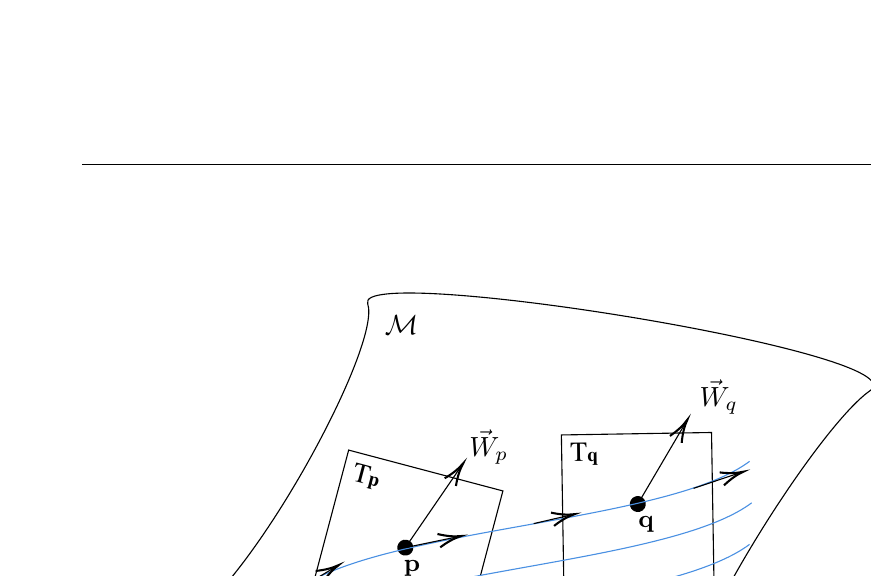
\begin{tikzpicture}[x=0.75pt,y=0.75pt,yscale=-1,xscale=1]
%uncomment if require: \path (0,290); %set diagram left start at 0, and has height of 290
%Shape: Square [id:dp9708989918743418] 
\draw   (186.51,80.08) -- (260.82,99.76) -- (241.13,174.07) -- (166.83,154.38) -- cycle ;
%Shape: Polygon Curved [id:ds40427350027465225] 
\draw   (195.67,9.5) .. controls (188.67,-10.5) and (463.67,33.5) .. (437.67,51.5) .. controls (411.67,69.5) and (338.67,185.5) .. (345.67,212.5) .. controls (352.67,239.5) and (71.67,183.5) .. (105.67,164.5) .. controls (139.67,145.5) and (202.67,29.5) .. (195.67,9.5) -- cycle ;
%Shape: Square [id:dp9131102785384768] 
\draw   (289,72.79) -- (361.34,71.6) -- (362.53,143.94) -- (290.19,145.13) -- cycle ;
%Straight Lines [id:da8576580265524865] 
\draw    (213.82,127.07) -- (240.53,88.15) ;
\draw [shift={(241.67,86.5)}, rotate = 484.46] [color={rgb, 255:red, 0; green, 0; blue, 0 }  ][line width=0.75]    (10.93,-3.29) .. controls (6.95,-1.4) and (3.31,-0.3) .. (0,0) .. controls (3.31,0.3) and (6.95,1.4) .. (10.93,3.29)   ;
\draw [shift={(213.82,127.07)}, rotate = 304.46] [color={rgb, 255:red, 0; green, 0; blue, 0 }  ][fill={rgb, 255:red, 0; green, 0; blue, 0 }  ][line width=0.75]      (0, 0) circle [x radius= 3.35, y radius= 3.35]   ;
%Straight Lines [id:da8303697446292895] 
\draw    (325.82,106.07) -- (348.65,67.22) ;
\draw [shift={(349.67,65.5)}, rotate = 480.44] [color={rgb, 255:red, 0; green, 0; blue, 0 }  ][line width=0.75]    (10.93,-3.29) .. controls (6.95,-1.4) and (3.31,-0.3) .. (0,0) .. controls (3.31,0.3) and (6.95,1.4) .. (10.93,3.29)   ;
\draw [shift={(325.82,106.07)}, rotate = 300.44] [color={rgb, 255:red, 0; green, 0; blue, 0 }  ][fill={rgb, 255:red, 0; green, 0; blue, 0 }  ][line width=0.75]      (0, 0) circle [x radius= 3.35, y radius= 3.35]   ;
%Curve Lines [id:da7066426387565043] 
\draw [color={rgb, 255:red, 74; green, 144; blue, 226 }  ,draw opacity=1 ]   (161.67,147.5) .. controls (170.02,141.23) and (182.65,136.19) .. (197.77,131.86) .. controls (255.04,115.44) and (348.02,109.23) .. (379.67,85.5) ;
%Straight Lines [id:da7306076516600093] 
\draw    (213.82,127.07) -- (238.71,121.91) ;
\draw [shift={(240.67,121.5)}, rotate = 528.27] [color={rgb, 255:red, 0; green, 0; blue, 0 }  ][line width=0.75]    (10.93,-3.29) .. controls (6.95,-1.4) and (3.31,-0.3) .. (0,0) .. controls (3.31,0.3) and (6.95,1.4) .. (10.93,3.29)   ;
%Straight Lines [id:da02716089781167641] 
\draw    (161.67,147.5) -- (179.95,136.53) ;
\draw [shift={(181.67,135.5)}, rotate = 509.04] [color={rgb, 255:red, 0; green, 0; blue, 0 }  ][line width=0.75]    (10.93,-3.29) .. controls (6.95,-1.4) and (3.31,-0.3) .. (0,0) .. controls (3.31,0.3) and (6.95,1.4) .. (10.93,3.29)   ;
%Straight Lines [id:da2970564313240187] 
\draw    (275.67,115.5) -- (293.43,111.4) ;
\draw [shift={(295.38,110.95)}, rotate = 527.01] [color={rgb, 255:red, 0; green, 0; blue, 0 }  ][line width=0.75]    (10.93,-3.29) .. controls (6.95,-1.4) and (3.31,-0.3) .. (0,0) .. controls (3.31,0.3) and (6.95,1.4) .. (10.93,3.29)   ;
%Straight Lines [id:da6321470360606996] 
\draw    (352.67,98.5) -- (374.77,91.13) ;
\draw [shift={(376.67,90.5)}, rotate = 521.5699999999999] [color={rgb, 255:red, 0; green, 0; blue, 0 }  ][line width=0.75]    (10.93,-3.29) .. controls (6.95,-1.4) and (3.31,-0.3) .. (0,0) .. controls (3.31,0.3) and (6.95,1.4) .. (10.93,3.29)   ;
%Curve Lines [id:da5314903136666809] 
\draw [color={rgb, 255:red, 74; green, 144; blue, 226 }  ,draw opacity=1 ]   (162.67,167.5) .. controls (171.02,161.23) and (183.65,156.19) .. (198.77,151.86) .. controls (256.04,135.44) and (349.02,129.23) .. (380.67,105.5) ;
%Curve Lines [id:da9023912184191769] 
\draw [color={rgb, 255:red, 74; green, 144; blue, 226 }  ,draw opacity=1 ]   (161.67,187.5) .. controls (170.02,181.23) and (182.65,176.19) .. (197.77,171.86) .. controls (255.04,155.44) and (348.02,149.23) .. (379.67,125.5) ;
% Text Node
\draw (217,137) node   [align=left] {\textbf{{\small p}}};
% Text Node
\draw (330,116) node   [align=left] {\textbf{{\small q}}};
% Text Node
\draw (212,20) node    {$\mathcal{M}$};
% Text Node
\draw (254,78.5) node   [align=left] {$\vec W_p$};
% Text Node
\draw (364.79,54.64) node   [align=left] {$\vec W_q$};
% Text Node
\draw (150,163) node  [color={rgb, 255:red, 74; green, 144; blue, 226 }  ,opacity=1 ] [align=left] {$\vec V$};
% Text Node
\draw (195,93) node  [rotate=-14.94] [align=left] {{\fontfamily{ptm}\selectfont T{\scriptsize \textbf{p}}}};
% Text Node
\draw (300,82) node  [rotate=-359.26] [align=left] {{\fontfamily{ptm}\selectfont T{\scriptsize \textbf{q}}}};
\end{tikzpicture}
        \caption{Manifold $\mathcal{M}$ with vector $\vec W$ changing from point \textbf{{\small p}} to point \textbf{{\small q}} along the flow lines of vector field $\vec V$} \label{Manifold}
            \end{center}
    \end{figure}
We need a way to compare $\vec W_q$ with $\vec W_p$ to make sense of a continuous change of $\vec W$ along the flow $\vec V$.  In flat space, we could simply take the difference of these two vectors and divide by the change in the parameter over that interval.  For more general curved space, we need a mathematical tool to "pull-back" $\vec W_q$ from the tangent plane at point \textbf{{\small q}} to the tangent plane at point \textbf{{\small p}} along the flow line of $\vec V$. Once we have pulled back $\vec W_q$ to the tangent plane at point \textbf{{\small p}}, we can then apply our standard calculus techniques on $\vec W_p$ and the pulled-back version of $\vec W_q$ because they both now belong to the same tangent space. The Lie derivative is the mathematical tool that will provide us what we need in the sense of pulling back a vector along the flow of another vector field so we can take the derivative of the vectors in the same tangent plane. 
The Lie derivative is a linear operator whose action on any $(k,l)$ tensor is given by:
\begin{equation}
\label{Lie tensor components}
   \mathcal{L}_{\vec V} \tensor {T}{^\mu_\nu} = V^\alpha \partial_\alpha \tensor{T}{^\mu_\nu} - \tensor {T}{^\alpha_\nu} \partial_\alpha V^\mu +\tensor{T}{^\mu_\alpha} \partial_\nu V^\alpha
\end{equation}
Equation (\ref{Lie tensor components}) shows that the Lie derivative is a linear map from $(k,l)$ tensors into $(k,l)$ tensors (even in curved spacetime). The Lie derivative obeys the Leibnez rule, which is essential to being a derivative operator:
\begin{equation}
\label{Leibnez Rule}
   \mathcal{L}_{\vec V} (T\otimes S) =(\mathcal{L}_{\vec V} T)\otimes S+T\otimes (\mathcal{L}_{\vec V} S)
\end{equation}
From (\ref{Lie tensor components}) we can derive the action of the Lie derivative on a vector:
\begin{equation}
\label{Lie vector}
   \mathcal{L}_{\vec V} W^\mu = V^\alpha \partial_\alpha W^\mu - W^\alpha \partial_\alpha V^\mu
\end{equation}
What we want is a directional derivative along $\vec V$, but the last term in (\ref{Lie vector}) is a derivative of the direction itself and therefore this equation will not be exactly what we are looking for in terms of a tensor calculus. As was shown in the homework, (\ref{Lie vector}) can be written in vector form using the Lie Bracket notation:
\begin{equation}
\label{Lie bracket}
   \mathcal{L}_{\vec V} \vec W = [\vec V,\vec W]=\vec V \vec W - \vec W \vec V
\end{equation}
It is not immediately clear how or why (\ref{Lie vector}) and (\ref{Lie bracket}) relate to the notion of the directional derivative of a vector. An analytical derivation showing how the Lie Bracket is related to the derivative of a vector along a flow curve will be provided at the end of this lecture, once the concepts of pullback and pushforward mappings have been introduced. In the meantime, the directional derivative aspect of the Lie derivative can be readily seen readily if we look at the action of the Lie derivative on a function using (\ref{Lie tensor components}):
\begin{equation}
\label{Lie function}
   \mathcal{L}_{\vec V} f = V^\alpha \partial_\alpha f
\end{equation}
So we see the Lie derivative acting on a function reduces down to our directional derivative notion of a "vector dotted with the gradient". We can also derive the action of the Lie derivative on a dual vector $\undertilde \omega = \omega_\nu \undertilde dx^\nu$ by using  (\ref{Lie tensor components}):
\begin{equation}
\label{Lie dual}
   (\mathcal{L}_{\vec V} \undertilde \omega) = (V^\alpha \partial_\alpha \omega_\nu +\omega_\alpha \partial_\nu V^\alpha) \undertilde dx^\nu
\end{equation}
Although (\ref{Lie dual}) is not very illuminating at this stage, it is important to notice the key differences between (\ref{Lie vector}) for a vector and (\ref{Lie dual}) for a dual vector.  In particular, the second term in the dual vector equation uses a plus sign as opposed to a minus sign for the vector equation.  Moreover, the Lie derivative of a dual vector involves only a single derivative of the flow field for each dual basis vector.$\\$
$\\$
Before proceeding any farther with the Lie derivative, we must introduce the pullback and pushforward mappings.

\newpage
     \subsection{General Pullback and Pushforward Mappings}
Let $\mathcal{M}$ and $\mathcal{N}$ be arbitrary manifolds and let $\phi : \mathcal{M} \longrightarrow \mathcal{N}$ be a smooth mapping of $\mathcal{M}$ into $\mathcal{N}$.  Let $f$ be a real-valued function on $\mathcal{N}$.  We define the pullback of $f$ onto $\mathcal{M}$, denoted $\phi^\ast$, to be (see Figure \ref{pullback}):
\begin{equation}
\label{pullback function equation}
   \phi^\ast f = f\circ \phi
\end{equation}
The pullback mapping works because we can compose $\phi : \mathcal{M} \longrightarrow \mathcal{N}$ with $f : \mathcal{N} \longrightarrow \mathbb{R}$ to obtain $\phi^\ast f =f\circ \phi: \mathcal{M} \longrightarrow \mathbb{R}$, which is a real-valued function on $\mathcal{M}$.  There is no way to "push-forward" a real-valued function on $\mathcal{M}$ into a real-valued function on $\mathcal{N}$ because our mapping $\phi$ is in one direction only (i.e., we can not devise a way to compose a real-valued function on $\mathcal{M}$ with the map $\phi$ to obtain a real-valued function on $\mathcal{N}$).  It should be intuitively obvious, however, that if $\phi$ is invertible then we would be able to "push-forward" a real-valued function on $\mathcal{M}$ into $\mathcal{N}$ by making use of $\phi^{-1}$, a fact we will return to in a bit.  
  \begin{figure} [H]
        \begin{center}
\tikzset{every picture/.style={line width=0.75pt}} %set default line width to 0.75pt        
\begin{tikzpicture}[x=0.75pt,y=0.75pt,yscale=-1,xscale=1]
%uncomment if require: \path (0,290); %set diagram left start at 0, and has height of 290
%Shape: Polygon Curved [id:ds5660253330347249] 
\draw   (84.5,57.33) .. controls (77.5,37.33) and (231.5,28.33) .. (205.5,46.33) .. controls (179.5,64.33) and (179.5,115.33) .. (186.5,142.33) .. controls (193.5,169.33) and (19.5,157.33) .. (53.5,138.33) .. controls (87.5,119.33) and (91.5,77.33) .. (84.5,57.33) -- cycle ;
%Shape: Polygon Curved [id:ds5100184750359966] 
\draw   (310.67,42.5) .. controls (344.5,19.33) and (430.5,21.33) .. (443.5,57.33) .. controls (456.5,93.33) and (419.5,115.33) .. (410.5,146.33) .. controls (401.5,177.33) and (293.5,146.33) .. (304.5,118.33) .. controls (315.5,90.33) and (276.83,65.67) .. (310.67,42.5) -- cycle ;
%Shape: Circle [id:dp058902741117860646] 
\draw  [color={rgb, 255:red, 0; green, 0; blue, 0 }  ,draw opacity=1 ][fill={rgb, 255:red, 0; green, 0; blue, 0 }  ,fill opacity=1 ] (133.37,94.45) .. controls (133.37,92.93) and (132.14,91.7) .. (130.62,91.7) .. controls (129.1,91.7) and (127.87,92.93) .. (127.87,94.45) .. controls (127.87,95.97) and (129.1,97.2) .. (130.62,97.2) .. controls (132.14,97.2) and (133.37,95.97) .. (133.37,94.45) -- cycle ;
%Shape: Circle [id:dp25289599168877763] 
\draw  [color={rgb, 255:red, 0; green, 0; blue, 0 }  ,draw opacity=1 ][fill={rgb, 255:red, 0; green, 0; blue, 0 }  ,fill opacity=1 ] (370.17,104.75) .. controls (370.17,102.96) and (368.71,101.5) .. (366.92,101.5) .. controls (365.12,101.5) and (363.67,102.96) .. (363.67,104.75) .. controls (363.67,106.54) and (365.12,108) .. (366.92,108) .. controls (368.71,108) and (370.17,106.54) .. (370.17,104.75) -- cycle ;
%Curve Lines [id:da6591700594059431] 
\draw    (138.5,92.33) .. controls (194.22,82.38) and (294.49,79.69) .. (359.52,98.38) ;
\draw [shift={(360.5,98.67)}, rotate = 196.29] [color={rgb, 255:red, 0; green, 0; blue, 0 }  ][line width=0.75]    (10.93,-3.29) .. controls (6.95,-1.4) and (3.31,-0.3) .. (0,0) .. controls (3.31,0.3) and (6.95,1.4) .. (10.93,3.29)   ;
%Shape: Square [id:dp9862702271371446] 
\draw   (321.25,199.08) -- (417.75,199.08) -- (417.75,295.58) -- (321.25,295.58) -- cycle ;
%Curve Lines [id:da7240076186277649] 
\draw    (372.5,116.33) .. controls (391.31,155.93) and (382.68,193.57) .. (370.86,237.02) ;
\draw [shift={(370.5,238.33)}, rotate = 285.26] [color={rgb, 255:red, 0; green, 0; blue, 0 }  ][line width=0.75]    (10.93,-3.29) .. controls (6.95,-1.4) and (3.31,-0.3) .. (0,0) .. controls (3.31,0.3) and (6.95,1.4) .. (10.93,3.29)   ;
%Shape: Circle [id:dp15835330722457153] 
\draw  [color={rgb, 255:red, 0; green, 0; blue, 0 }  ,draw opacity=1 ][fill={rgb, 255:red, 0; green, 0; blue, 0 }  ,fill opacity=1 ] (369.5,247.33) .. controls (369.5,245.54) and (368.04,244.08) .. (366.25,244.08) .. controls (364.46,244.08) and (363,245.54) .. (363,247.33) .. controls (363,249.13) and (364.46,250.58) .. (366.25,250.58) .. controls (368.04,250.58) and (369.5,249.13) .. (369.5,247.33) -- cycle ;
%Curve Lines [id:da7793678595204823] 
\draw    (135.5,105.33) .. controls (161.87,150.19) and (286.25,233.5) .. (354.48,245.16) ;
\draw [shift={(355.5,245.33)}, rotate = 189.19] [color={rgb, 255:red, 0; green, 0; blue, 0 }  ][line width=0.75]    (10.93,-3.29) .. controls (6.95,-1.4) and (3.31,-0.3) .. (0,0) .. controls (3.31,0.3) and (6.95,1.4) .. (10.93,3.29)   ;
% Text Node
\draw (100,60) node    {$\mathcal{M}$};
% Text Node
\draw (325,50) node    {$\mathcal{N}$};
% Text Node
\draw (247,71) node    {$\phi$};
% Text Node
\draw (119.8,94.1) node   [align=left] {\textbf{{\small p}}};
% Text Node
\draw (387,104.5) node   [align=left] {{$\phi$}({\textbf{{\small p}}})};
% Text Node
\draw (394,176) node    {$f$};
% Text Node
\draw (196.5,202.5) node    {$\phi^\ast f = f\circ \phi$};
% Text Node
\draw (410,210) node    {$\mathbb{R}$};
\end{tikzpicture}
        \caption{Pullback mapping of a real-valued function on manifold $\mathcal{N}$ to a real-valued function on manifold $\mathcal{M}$} \label{pullback}
            \end{center}
    \end{figure}
Functions \textbf{can not} be pushed forward for a general $\phi$ mapping of $\mathcal{M}$ into $\mathcal{N}$ because the composition does not work properly. Vectors, on the other hand, can be pushed forward from $\mathcal{M}$ into $\mathcal{N}$ because of how they act on functions. Specifically, we define the pushforward of $\vec V$ from the tangent space of point \textbf{{\small p}} in $\mathcal{M}$ to the tangent space of point $\phi (\textbf{{\small p}})$ in $\mathcal{N}$ as follows:
\begin{equation}
\label{pushforward vector equation}
   \phi_\ast \vec V (f)= \vec V (\phi^\ast f)
\end{equation}
Equation (\ref {pushforward vector equation}) is shown graphically in Figure \ref{pushforward}.  Notice that (\ref {pushforward vector equation}) makes sense from a functional perspective by examining each of the objects being mapped and the space they reside in, as shown below.
        \begin{center}
\tikzset{every picture/.style={line width=0.75pt}} %set default line width to 0.75pt        
\begin{tikzpicture}[x=0.75pt,y=0.75pt,yscale=-1,xscale=1]
%uncomment if require: \path (0,300); %set diagram left start at 0, and has height of 300
%Shape: Brace [id:dp5871599193459534] 
\draw   (98.4,122.27) .. controls (98.44,126.94) and (100.79,129.25) .. (105.46,129.2) -- (110.86,129.16) .. controls (117.53,129.1) and (120.88,131.4) .. (120.92,136.07) .. controls (120.88,131.4) and (124.19,129.04) .. (130.86,128.98)(127.86,129) -- (136.26,128.93) .. controls (140.93,128.89) and (143.24,126.54) .. (143.2,121.87) ;
%Shape: Brace [id:dp9454920969779972] 
\draw   (190.4,105.07) .. controls (190.37,100.4) and (188.03,98.08) .. (183.36,98.11) -- (178.91,98.14) .. controls (172.24,98.18) and (168.89,95.87) .. (168.86,91.2) .. controls (168.89,95.87) and (165.58,98.22) .. (158.91,98.26)(161.91,98.25) -- (154.46,98.29) .. controls (149.79,98.32) and (147.47,100.67) .. (147.5,105.34) ;
%Shape: Brace [id:dp7771032990307483] 
\draw   (218.1,121.53) .. controls (218.1,126.2) and (220.43,128.53) .. (225.1,128.53) -- (225.6,128.53) .. controls (232.27,128.53) and (235.6,130.86) .. (235.6,135.53) .. controls (235.6,130.86) and (238.93,128.53) .. (245.6,128.53)(242.6,128.53) -- (246.1,128.53) .. controls (250.77,128.53) and (253.1,126.2) .. (253.1,121.53) ;
%Shape: Brace [id:dp06589976628708105] 
\draw   (300.1,105.13) .. controls (300.1,100.46) and (297.77,98.13) .. (293.1,98.13) -- (285.6,98.13) .. controls (278.93,98.13) and (275.6,95.8) .. (275.6,91.13) .. controls (275.6,95.8) and (272.27,98.13) .. (265.6,98.13)(268.6,98.13) -- (258.1,98.13) .. controls (253.43,98.13) and (251.1,100.46) .. (251.1,105.13) ;
% Text Node
\draw (199,113) node    {$\Phi_\ast \vec V\ \ \ ( \ \ f\ \ ) \ \ \ =\ \ \ \vec V\ \ \ ( \Phi^\ast f)$};
% Text Node
\draw (121.2,143.8) node   [align=left] {{\small Vector in $\mathcal{N}$}};
% Text Node
\draw (176,82.4) node   [align=left] {{\small Function on $\mathcal{N}$}};
% Text Node
\draw (238.8,143) node   [align=left] {{\small Vector in $\mathcal{M}$}};
% Text Node
\draw (286.2,82) node   [align=left] {{\small Function on $\mathcal{M}$}};
\end{tikzpicture}
 \end{center}

  \begin{figure} [H]
        \begin{center}
\tikzset{every picture/.style={line width=0.75pt}} %set default line width to 0.75pt        
\begin{tikzpicture}[x=0.75pt,y=0.75pt,yscale=-1,xscale=1]
%uncomment if require: \path (0,290); %set diagram left start at 0, and has height of 290
%Shape: Polygon Curved [id:ds16994228869089634] 
\draw   (104.5,51.75) .. controls (97.5,31.75) and (251.5,22.75) .. (225.5,40.75) .. controls (199.5,58.75) and (199.5,109.75) .. (206.5,136.75) .. controls (213.5,163.75) and (39.5,151.75) .. (73.5,132.75) .. controls (107.5,113.75) and (111.5,71.75) .. (104.5,51.75) -- cycle ;
%Shape: Polygon Curved [id:ds9276705934056806] 
\draw   (330.67,36.92) .. controls (364.5,13.75) and (450.5,15.75) .. (463.5,51.75) .. controls (476.5,87.75) and (439.5,109.75) .. (430.5,140.75) .. controls (421.5,171.75) and (313.5,140.75) .. (324.5,112.75) .. controls (335.5,84.75) and (296.83,60.08) .. (330.67,36.92) -- cycle ;
%Shape: Circle [id:dp017263383869670523] 
\draw  [color={rgb, 255:red, 0; green, 0; blue, 0 }  ,draw opacity=1 ][fill={rgb, 255:red, 0; green, 0; blue, 0 }  ,fill opacity=1 ] (153.37,88.87) .. controls (153.37,87.35) and (152.14,86.12) .. (150.62,86.12) .. controls (149.1,86.12) and (147.87,87.35) .. (147.87,88.87) .. controls (147.87,90.39) and (149.1,91.62) .. (150.62,91.62) .. controls (152.14,91.62) and (153.37,90.39) .. (153.37,88.87) -- cycle ;
%Shape: Circle [id:dp8676399248895204] 
\draw  [color={rgb, 255:red, 0; green, 0; blue, 0 }  ,draw opacity=1 ][fill={rgb, 255:red, 0; green, 0; blue, 0 }  ,fill opacity=1 ] (390.17,99.17) .. controls (390.17,97.37) and (388.71,95.92) .. (386.92,95.92) .. controls (385.12,95.92) and (383.67,97.37) .. (383.67,99.17) .. controls (383.67,100.96) and (385.12,102.42) .. (386.92,102.42) .. controls (388.71,102.42) and (390.17,100.96) .. (390.17,99.17) -- cycle ;
%Curve Lines [id:da8722914481639557] 
\draw    (158.5,86.75) .. controls (214.22,76.8) and (314.49,74.11) .. (379.52,92.8) ;
\draw [shift={(380.5,93.08)}, rotate = 196.29] [color={rgb, 255:red, 0; green, 0; blue, 0 }  ][line width=0.75]    (10.93,-3.29) .. controls (6.95,-1.4) and (3.31,-0.3) .. (0,0) .. controls (3.31,0.3) and (6.95,1.4) .. (10.93,3.29)   ;
%Shape: Square [id:dp9050807835893067] 
\draw   (341.25,193.5) -- (437.75,193.5) -- (437.75,290) -- (341.25,290) -- cycle ;
%Curve Lines [id:da9416749225577381] 
\draw    (392.5,110.75) .. controls (411.31,150.35) and (402.68,187.99) .. (390.86,231.43) ;
\draw [shift={(390.5,232.75)}, rotate = 285.26] [color={rgb, 255:red, 0; green, 0; blue, 0 }  ][line width=0.75]    (10.93,-3.29) .. controls (6.95,-1.4) and (3.31,-0.3) .. (0,0) .. controls (3.31,0.3) and (6.95,1.4) .. (10.93,3.29)   ;
%Shape: Circle [id:dp7624827425768117] 
\draw  [color={rgb, 255:red, 0; green, 0; blue, 0 }  ,draw opacity=1 ][fill={rgb, 255:red, 0; green, 0; blue, 0 }  ,fill opacity=1 ] (389.5,241.75) .. controls (389.5,239.96) and (388.04,238.5) .. (386.25,238.5) .. controls (384.46,238.5) and (383,239.96) .. (383,241.75) .. controls (383,243.54) and (384.46,245) .. (386.25,245) .. controls (388.04,245) and (389.5,243.54) .. (389.5,241.75) -- cycle ;
%Curve Lines [id:da8684186844388702] 
\draw    (155.5,99.75) .. controls (181.87,144.61) and (306.25,227.91) .. (374.48,239.58) ;
\draw [shift={(375.5,239.75)}, rotate = 189.19] [color={rgb, 255:red, 0; green, 0; blue, 0 }  ][line width=0.75]    (10.93,-3.29) .. controls (6.95,-1.4) and (3.31,-0.3) .. (0,0) .. controls (3.31,0.3) and (6.95,1.4) .. (10.93,3.29)   ;
%Shape: Square [id:dp7834174223472223] 
\draw   (131.04,57.93) -- (184.3,72.04) -- (170.19,125.3) -- (116.93,111.19) -- cycle ;
%Shape: Square [id:dp830268997283313] 
\draw   (362.47,68.84) -- (417.25,74.72) -- (411.36,129.5) -- (356.59,123.61) -- cycle ;
%Straight Lines [id:da37124461036035883] 
\draw    (151.62,88.12) -- (174.79,74.04) ;
\draw [shift={(176.5,73)}, rotate = 508.72] [color={rgb, 255:red, 0; green, 0; blue, 0 }  ][line width=0.75]    (10.93,-3.29) .. controls (6.95,-1.4) and (3.31,-0.3) .. (0,0) .. controls (3.31,0.3) and (6.95,1.4) .. (10.93,3.29)   ;
%Straight Lines [id:da7736234404432303] 
\draw    (386.92,99.17) -- (405.98,67.18) ;
\draw [shift={(407,65.47)}, rotate = 480.79] [color={rgb, 255:red, 0; green, 0; blue, 0 }  ][line width=0.75]    (10.93,-3.29) .. controls (6.95,-1.4) and (3.31,-0.3) .. (0,0) .. controls (3.31,0.3) and (6.95,1.4) .. (10.93,3.29)   ;
% Text Node
\draw (120,54.42) node    {$\mathcal{M}$};
% Text Node
\draw (345,44.42) node    {$\mathcal{N}$};
% Text Node
\draw (267,65.42) node    {$\phi_\ast$};
% Text Node
\draw (139.8,88.52) node   [align=left] {$\vec V$};
% Text Node
\draw (400,103.92) node   [align=left] {{$\phi_\ast$}{$\vec V$}};
% Text Node
\draw (432,170.42) node    {({$\phi_\ast$}{$\vec V$})({$f$})};
% Text Node
\draw (225,196.92) node    {{$\vec V$}({$\phi^\ast f$})};
% Text Node
\draw (430,202) node    {$\mathbb{R}$};
\end{tikzpicture}
        \caption{Pushforward mapping of a vector in manifold $\mathcal{M}$ to a vector in manifold $\mathcal{N}$} \label{pushforward}
            \end{center}
    \end{figure}
Now that we have defined a method to pushforward vectors, the next logical step is to figure out what we can do with dual vectors. Functions can be pulled back because of how they compose, and vectors can be pushed forward because of how they act on functions.  Since dual vectors act on vectors (and viewing a function as a $0$-form), it is reasonable to guess that a pullback mapping can be defined for dual vectors. Indeed, for $\undertilde \omega = \omega_\nu \undertilde dx^\nu$ in $\mathcal{N}$ we have the pullback of a dual vector from $\mathcal{N}$ to $\mathcal{M}$ given by:
\begin{equation}
\label{pullback dual equation}
   \phi^\ast \undertilde \omega (\vec V) = \undertilde \omega (\phi_\ast \vec V)
\end{equation}
Again, we can ensure (\ref {pullback dual equation}) makes sense from a functional perspective by examining each of the objects being mapped and the space they reside in, as shown below.
        \begin{center}
\tikzset{every picture/.style={line width=0.75pt}} %set default line width to 0.75pt        
\begin{tikzpicture}[x=0.75pt,y=0.75pt,yscale=-1,xscale=1]
%uncomment if require: \path (0,300); %set diagram left start at 0, and has height of 300
%Shape: Brace [id:dp5871599193459534] 
\draw   (98.4,122.27) .. controls (98.44,126.94) and (100.79,129.25) .. (105.46,129.2) -- (110.86,129.16) .. controls (117.53,129.1) and (120.88,131.4) .. (120.92,136.07) .. controls (120.88,131.4) and (124.19,129.04) .. (130.86,128.98)(127.86,129) -- (136.26,128.93) .. controls (140.93,128.89) and (143.24,126.54) .. (143.2,121.87) ;
%Shape: Brace [id:dp9454920969779972] 
\draw   (190.4,105.07) .. controls (190.37,100.4) and (188.03,98.08) .. (183.36,98.11) -- (178.91,98.14) .. controls (172.24,98.18) and (168.89,95.87) .. (168.86,91.2) .. controls (168.89,95.87) and (165.58,98.22) .. (158.91,98.26)(161.91,98.25) -- (154.46,98.29) .. controls (149.79,98.32) and (147.47,100.67) .. (147.5,105.34) ;
%Shape: Brace [id:dp7771032990307483] 
\draw   (218.1,121.53) .. controls (218.1,126.2) and (220.43,128.53) .. (225.1,128.53) -- (225.6,128.53) .. controls (232.27,128.53) and (235.6,130.86) .. (235.6,135.53) .. controls (235.6,130.86) and (238.93,128.53) .. (245.6,128.53)(242.6,128.53) -- (246.1,128.53) .. controls (250.77,128.53) and (253.1,126.2) .. (253.1,121.53) ;
%Shape: Brace [id:dp06589976628708105] 
\draw   (300.1,105.13) .. controls (300.1,100.46) and (297.77,98.13) .. (293.1,98.13) -- (285.6,98.13) .. controls (278.93,98.13) and (275.6,95.8) .. (275.6,91.13) .. controls (275.6,95.8) and (272.27,98.13) .. (265.6,98.13)(268.6,98.13) -- (258.1,98.13) .. controls (253.43,98.13) and (251.1,100.46) .. (251.1,105.13) ;
% Text Node
\draw (199,113) node    {$\phi^\ast \undertilde \omega\ \ \ ( \ \ \vec V\ \ ) \ \ \ =\ \ \ \undertilde \omega\ \ \ (\phi_\ast \vec V)$};
% Text Node
\draw (121.2,143.8) node   [align=left] {{\small Dual vector in $\mathcal{M}$}};
% Text Node
\draw (176,82.4) node   [align=left] {{\small Vector in $\mathcal{M}$}};
% Text Node
\draw (238.8,143) node   [align=left] {{\small Dual vector in $\mathcal{N}$}};
% Text Node
\draw (286.2,82) node   [align=left] {{\small Vector in $\mathcal{N}$}};
\end{tikzpicture}
 \end{center}
We can pullback functions and dual vectors, and we can pushforward vectors.  Can we generalize this to arbitrary tensors?  Turns out that, without placing additional structure on $\phi: \mathcal{M} \longrightarrow \mathcal{N}$, the most general operations we can do are: 
\begin{center}
\textbf{Pushforward $(k,0)$ tensors}\\
\textbf{Pullback $(0,l)$ tensors}
 \end{center}
The definitions of pullback and pushforward mappings are abstract at this time because we are working with the geometric objects associated with manifolds $\mathcal{M}$ and $\mathcal{N}$. In order to analyze these definitions more carefully, we need to provide coordinates $x^\mu$ and $y^\alpha$ for $\mathcal{M}$ and $\mathcal{N}$, respectively.  Remember that coordinates are really defined locally on $\mathbb{R}^n$ via a chart but we do not need that additional level of detail at this time. Also, in the most general setting $\mathcal{M}$ and $\mathcal{N}$ may have different dimensions so our coordinates may come from entirely different euclidean spaces.
With coordinates defined on $\mathcal{M}$ and $\mathcal{N}$, we can associated our original mapping $\phi$ with a vector-valued function $\vec y:\mathbb{R}^m \longrightarrow \mathbb{R}^n$ where $m=$\ dim($\mathcal{M}$), $n= $\ dim($\mathcal{N}$), and $\vec y=(y^0 (x^0,...,x^m),y^1 (x^0,...,x^m),...,y^n(x^0,...,x^m))$.  Note that the components of $\vec y$ are just $y^\alpha (x^\mu)$. So in coordinate notation the pullback of a function given by (\ref {pullback function equation}) becomes:
\begin{equation}
\label{pullback function components}
   \phi^\ast f = f\circ \phi = f(y^\alpha(x^\mu))\\
\end{equation} 
The pushforward of a vector given by (\ref {pushforward vector equation}) becomes:
\begin{equation}
\label{pushforward vector components1}
    \vec V (\phi^\ast f)=V^\mu \partial_\mu (f(y^\alpha(x^\mu)))=V^\mu \frac{\partial f}{\partial y^\alpha} \frac{\partial y^\alpha}{\partial x^\mu}
\end{equation} 
But notice we can also express (\ref {pushforward vector equation}) in coordinate notation as:
\begin{equation}
\label{pushforward vector components2}
   \phi_\ast \vec V (f)= (\phi_\ast \vec V)^\alpha \partial_\alpha (f(y^\alpha(x^\mu)))= (\phi_\ast \vec V)^\alpha  \frac{\partial f}{\partial y^\alpha}
\end{equation}
These two equations must be equivalent, which gives us the following relationship:
\begin{equation}
\label{pushforward vector components3}
    (\phi_\ast \vec V)^\alpha = V^\mu  \frac{\partial y^\alpha}{\partial x^\mu} = \frac{\partial y^\alpha}{\partial x^\mu}  V^\mu
\end{equation}
So our pushforward mapping of vector $\vec V$ can be expressed as a matrix acting on $\vec V$, with the transformation matrix defined by:
\begin{equation}
\label{pushforward vector components4}
    \tensor{(\phi_\ast)}{^\alpha_\mu} = \frac{\partial y^\alpha}{\partial x^\mu}
\end{equation}
Transformation matrix  (\ref {pushforward vector components4}) is an $m \cross n$ matrix where $m=$\ dim($\mathcal{M}$) $n= $\ dim($\mathcal{N}$) as previously noted. In the special case where $m=n$ and the inverse matrix exists, we can define a pullback of a vector in a natural way (i.e., by pushing forward the inverse mapping). This concept is explored in more detail in the following section.

\newpage
     \subsection{Invertible Pullback and Pushforward Mappings}
Invertible mappings play a crucial role in the analysis of the Lie derivative because we need to compare vectors from the tangent planes of two nearby point in the same manifold. So we are most interested in mappings $\phi : \mathcal{M} \longrightarrow \mathcal{M}$, which means transformation matrix (\ref {pushforward vector components4}) will be an $m \cross m$ matrix.  Moreover, the notion of a derivative means our two points should be "infinitesimally" close to each other, so we can linearize our mapping $\phi$ in the region of the two points on $\mathcal{M}$, thereby allowing us to locally define $\phi^{-1} : \mathcal{M} \longrightarrow \mathcal{M}$.\footnote{A smooth, invertible map $\phi : \mathcal{M} \longrightarrow \mathcal{N}$ is called a diffeomorphism.  By smooth, we mean that when we write the mapping in terms of component functions $y^\alpha (x^\mu)$, these functions can be differentiated in the usual calculus sense. If a diffeomorphism exists between manifold $\mathcal{M}$ and $\mathcal{N}$, we say $\mathcal{M}$ and $\mathcal{N}$ are diffeomorphic written as $\mathcal{M} \cong \mathcal{N}$.  Diffeomorphic manifolds are essentially the same manifold.} Using $\phi^{-1}$, we can define what is meant by the pullback of a vector:
\begin{equation}
\label{pullback vector equation}
   \phi^\ast \vec V (f)= \phi_\ast^{-1} \vec V (f) = \vec V (\phi^{\ast -1} f)=\vec V(f \circ \phi^{-1})
\end{equation}
Similarly, we can use $\phi^{-1}$ to define the pushforward of a dual vector. Once pullbacks and pushforwards are defined for both vectors and dual vectors, we can then define the pullback and pushforward of a general tensor. Since the Lie derivative does not require this much mathematical machinery, we will only need the pushforward and pullback of a vector at this time.

We can illustrate the example of an invertible, smooth mapping of manifolds by looking at the case of the 2-Sphere $\mathcal{S}^2$ with $\vec V=\vec \partial_\phi$. Then our mapping $\phi:\mathcal{S}^2 \longrightarrow \mathcal{S}^2$ will move points around on $\mathcal{S}^2$ in the direction of $\vec \phi$. The flow lines are lines of constant lattitude, with each curve representing a fixed value of $\theta$. We can express these smooth curves as $\phi(\lambda)$, and this mapping is clearly invertible by reversing the direction of travel (from clockwise to counter clockwise or vice-versa).  These concepts are shown in Figure \ref{2-sphere}.
    \begin{figure} [H]
        \begin{center}
\tikzset{every picture/.style={line width=0.75pt}} %set default line width to 0.75pt        
\begin{tikzpicture}[x=0.75pt,y=0.75pt,yscale=-1,xscale=1]
%uncomment if require: \path (0,290); %set diagram left start at 0, and has height of 290
%Shape: Circle [id:dp11835659593105397] 
\draw   (100,179.75) .. controls (100,138.47) and (133.47,105) .. (174.75,105) .. controls (216.03,105) and (249.5,138.47) .. (249.5,179.75) .. controls (249.5,221.03) and (216.03,254.5) .. (174.75,254.5) .. controls (133.47,254.5) and (100,221.03) .. (100,179.75) -- cycle ;
%Shape: Arc [id:dp3569608368355768] 
\draw  [draw opacity=0][dash pattern={on 4.5pt off 4.5pt}] (243.65,159.83) .. controls (246.97,164.12) and (248.57,168.87) .. (248.06,173.87) .. controls (246.03,193.71) and (211.59,210.04) .. (171.13,210.34) .. controls (130.67,210.64) and (99.52,194.81) .. (101.55,174.97) .. controls (102.1,169.63) and (104.98,164.55) .. (109.7,159.97) -- (174.8,174.42) -- cycle ; \draw  [color={rgb, 255:red, 74; green, 144; blue, 226 }  ,draw opacity=1 ][dash pattern={on 4.5pt off 4.5pt}] (243.65,159.83) .. controls (246.97,164.12) and (248.57,168.87) .. (248.06,173.87) .. controls (246.03,193.71) and (211.59,210.04) .. (171.13,210.34) .. controls (130.67,210.64) and (99.52,194.81) .. (101.55,174.97) .. controls (102.1,169.63) and (104.98,164.55) .. (109.7,159.97) ;
%Shape: Arc [id:dp3048115149392767] 
\draw  [draw opacity=0][dash pattern={on 4.5pt off 4.5pt}] (230.08,137.07) .. controls (238.85,141.42) and (243.84,147.02) .. (243.36,153.26) .. controls (242.21,168.15) and (210.25,180.97) .. (171.98,181.89) .. controls (133.7,182.82) and (103.6,171.49) .. (104.75,156.6) .. controls (105.19,150.87) and (110.18,145.45) .. (118.34,140.89) -- (174.05,154.93) -- cycle ; \draw  [color={rgb, 255:red, 74; green, 144; blue, 226 }  ,draw opacity=1 ][dash pattern={on 4.5pt off 4.5pt}] (230.08,137.07) .. controls (238.85,141.42) and (243.84,147.02) .. (243.36,153.26) .. controls (242.21,168.15) and (210.25,180.97) .. (171.98,181.89) .. controls (133.7,182.82) and (103.6,171.49) .. (104.75,156.6) .. controls (105.19,150.87) and (110.18,145.45) .. (118.34,140.89) ;
%Shape: Arc [id:dp22397045221348866] 
\draw  [draw opacity=0][dash pattern={on 4.5pt off 4.5pt}] (244.53,204.47) .. controls (244.56,205.07) and (244.55,205.68) .. (244.48,206.29) .. controls (242.92,221.56) and (211.46,234.44) .. (174.21,235.07) .. controls (136.96,235.69) and (108.03,223.82) .. (109.59,208.55) .. controls (109.74,207.14) and (110.14,205.75) .. (110.77,204.39) -- (177.04,207.42) -- cycle ; \draw  [color={rgb, 255:red, 74; green, 144; blue, 226 }  ,draw opacity=1 ][dash pattern={on 4.5pt off 4.5pt}] (244.53,204.47) .. controls (244.56,205.07) and (244.55,205.68) .. (244.48,206.29) .. controls (242.92,221.56) and (211.46,234.44) .. (174.21,235.07) .. controls (136.96,235.69) and (108.03,223.82) .. (109.59,208.55) .. controls (109.74,207.14) and (110.14,205.75) .. (110.77,204.39) ;
%Shape: Arc [id:dp5807756495866188] 
\draw  [draw opacity=0][dash pattern={on 4.5pt off 4.5pt}] (214.47,121.09) .. controls (225.2,124.4) and (231.67,129.3) .. (231.24,134.91) .. controls (230.41,145.76) and (204.07,155.17) .. (172.41,155.93) .. controls (140.75,156.69) and (115.76,148.52) .. (116.6,137.67) .. controls (117.02,132.2) and (123.91,127.1) .. (134.7,123.29) -- (173.92,136.29) -- cycle ; \draw  [color={rgb, 255:red, 74; green, 144; blue, 226 }  ,draw opacity=1 ][dash pattern={on 4.5pt off 4.5pt}] (214.47,121.09) .. controls (225.2,124.4) and (231.67,129.3) .. (231.24,134.91) .. controls (230.41,145.76) and (204.07,155.17) .. (172.41,155.93) .. controls (140.75,156.69) and (115.76,148.52) .. (116.6,137.67) .. controls (117.02,132.2) and (123.91,127.1) .. (134.7,123.29) ;
%Shape: Arc [id:dp5470309612863797] 
\draw  [draw opacity=0][dash pattern={on 4.5pt off 4.5pt}] (199.76,109.06) .. controls (204.48,111.31) and (207.21,114.33) .. (206.95,117.71) .. controls (206.38,125.17) and (191.43,131.57) .. (173.57,132) .. controls (155.71,132.43) and (141.7,126.73) .. (142.27,119.27) .. controls (142.52,115.99) and (145.55,112.91) .. (150.39,110.46) -- (174.61,118.49) -- cycle ; \draw  [color={rgb, 255:red, 74; green, 144; blue, 226 }  ,draw opacity=1 ][dash pattern={on 4.5pt off 4.5pt}] (199.76,109.06) .. controls (204.48,111.31) and (207.21,114.33) .. (206.95,117.71) .. controls (206.38,125.17) and (191.43,131.57) .. (173.57,132) .. controls (155.71,132.43) and (141.7,126.73) .. (142.27,119.27) .. controls (142.52,115.99) and (145.55,112.91) .. (150.39,110.46) ;
%Straight Lines [id:da480389364348875] 
\draw    (114.67,170.67) -- (128.94,176.87) ;
\draw [shift={(130.78,177.67)}, rotate = 203.48] [color={rgb, 255:red, 0; green, 0; blue, 0 }  ][line width=0.75]    (10.93,-3.29) .. controls (6.95,-1.4) and (3.31,-0.3) .. (0,0) .. controls (3.31,0.3) and (6.95,1.4) .. (10.93,3.29)   ;
%Straight Lines [id:da39657874155740447] 
\draw    (151.33,181) -- (166.12,182.47) ;
\draw [shift={(168.11,182.67)}, rotate = 185.67] [color={rgb, 255:red, 0; green, 0; blue, 0 }  ][line width=0.75]    (10.93,-3.29) .. controls (6.95,-1.4) and (3.31,-0.3) .. (0,0) .. controls (3.31,0.3) and (6.95,1.4) .. (10.93,3.29)   ;
%Straight Lines [id:da6396416977572423] 
\draw    (191.33,180) -- (205.47,177.95) ;
\draw [shift={(207.44,177.67)}, rotate = 531.76] [color={rgb, 255:red, 0; green, 0; blue, 0 }  ][line width=0.75]    (10.93,-3.29) .. controls (6.95,-1.4) and (3.31,-0.3) .. (0,0) .. controls (3.31,0.3) and (6.95,1.4) .. (10.93,3.29)   ;
%Straight Lines [id:da21001080369805214] 
\draw    (226,170) -- (237.73,163.02) ;
\draw [shift={(239.44,162)}, rotate = 509.25] [color={rgb, 255:red, 0; green, 0; blue, 0 }  ][line width=0.75]    (10.93,-3.29) .. controls (6.95,-1.4) and (3.31,-0.3) .. (0,0) .. controls (3.31,0.3) and (6.95,1.4) .. (10.93,3.29)   ;
%Straight Lines [id:da3096937371399049] 
\draw    (112.67,196.67) -- (125,203.08) ;
\draw [shift={(126.78,204)}, rotate = 207.46] [color={rgb, 255:red, 0; green, 0; blue, 0 }  ][line width=0.75]    (10.93,-3.29) .. controls (6.95,-1.4) and (3.31,-0.3) .. (0,0) .. controls (3.31,0.3) and (6.95,1.4) .. (10.93,3.29)   ;
%Straight Lines [id:da6841438447454484] 
\draw    (146.67,208.67) -- (159.48,210.98) ;
\draw [shift={(161.44,211.33)}, rotate = 190.23] [color={rgb, 255:red, 0; green, 0; blue, 0 }  ][line width=0.75]    (10.93,-3.29) .. controls (6.95,-1.4) and (3.31,-0.3) .. (0,0) .. controls (3.31,0.3) and (6.95,1.4) .. (10.93,3.29)   ;
%Straight Lines [id:da7187750015844925] 
\draw    (185.33,209.33) -- (198.13,207.6) ;
\draw [shift={(200.11,207.33)}, rotate = 532.29] [color={rgb, 255:red, 0; green, 0; blue, 0 }  ][line width=0.75]    (10.93,-3.29) .. controls (6.95,-1.4) and (3.31,-0.3) .. (0,0) .. controls (3.31,0.3) and (6.95,1.4) .. (10.93,3.29)   ;
%Straight Lines [id:da6255611716804006] 
\draw    (221.33,200.67) -- (234.29,194.82) ;
\draw [shift={(236.11,194)}, rotate = 515.72] [color={rgb, 255:red, 0; green, 0; blue, 0 }  ][line width=0.75]    (10.93,-3.29) .. controls (6.95,-1.4) and (3.31,-0.3) .. (0,0) .. controls (3.31,0.3) and (6.95,1.4) .. (10.93,3.29)   ;
%Straight Lines [id:da6237571999775042] 
\draw    (130,228.67) -- (142.21,232.71) ;
\draw [shift={(144.11,233.33)}, rotate = 198.3] [color={rgb, 255:red, 0; green, 0; blue, 0 }  ][line width=0.75]    (10.93,-3.29) .. controls (6.95,-1.4) and (3.31,-0.3) .. (0,0) .. controls (3.31,0.3) and (6.95,1.4) .. (10.93,3.29)   ;
%Straight Lines [id:da6337912780871908] 
\draw    (170,235.33) -- (183.44,235.33) ;
\draw [shift={(185.44,235.33)}, rotate = 540] [color={rgb, 255:red, 0; green, 0; blue, 0 }  ][line width=0.75]    (10.93,-3.29) .. controls (6.95,-1.4) and (3.31,-0.3) .. (0,0) .. controls (3.31,0.3) and (6.95,1.4) .. (10.93,3.29)   ;
%Straight Lines [id:da028879191732378295] 
\draw    (207.33,230.67) -- (220.18,227.19) ;
\draw [shift={(222.11,226.67)}, rotate = 524.85] [color={rgb, 255:red, 0; green, 0; blue, 0 }  ][line width=0.75]    (10.93,-3.29) .. controls (6.95,-1.4) and (3.31,-0.3) .. (0,0) .. controls (3.31,0.3) and (6.95,1.4) .. (10.93,3.29)   ;
%Straight Lines [id:da6794640500652227] 
\draw    (121.67,146.67) -- (135.6,152.55) ;
\draw [shift={(137.44,153.33)}, rotate = 202.91] [color={rgb, 255:red, 0; green, 0; blue, 0 }  ][line width=0.75]    (10.93,-3.29) .. controls (6.95,-1.4) and (3.31,-0.3) .. (0,0) .. controls (3.31,0.3) and (6.95,1.4) .. (10.93,3.29)   ;
%Straight Lines [id:da7213353963898663] 
\draw    (159.67,156) -- (175.44,156) ;
\draw [shift={(177.44,156)}, rotate = 540] [color={rgb, 255:red, 0; green, 0; blue, 0 }  ][line width=0.75]    (10.93,-3.29) .. controls (6.95,-1.4) and (3.31,-0.3) .. (0,0) .. controls (3.31,0.3) and (6.95,1.4) .. (10.93,3.29)   ;
%Straight Lines [id:da4720025228427165] 
\draw    (201,153) -- (217.51,148.82) ;
\draw [shift={(219.44,148.33)}, rotate = 525.8] [color={rgb, 255:red, 0; green, 0; blue, 0 }  ][line width=0.75]    (10.93,-3.29) .. controls (6.95,-1.4) and (3.31,-0.3) .. (0,0) .. controls (3.31,0.3) and (6.95,1.4) .. (10.93,3.29)   ;
%Straight Lines [id:da0933393043342079] 
\draw    (144,124) -- (156.99,130.44) ;
\draw [shift={(158.78,131.33)}, rotate = 206.39] [color={rgb, 255:red, 0; green, 0; blue, 0 }  ][line width=0.75]    (10.93,-3.29) .. controls (6.95,-1.4) and (3.31,-0.3) .. (0,0) .. controls (3.31,0.3) and (6.95,1.4) .. (10.93,3.29)   ;
%Straight Lines [id:da02307575447616017] 
\draw    (182.67,131.33) -- (196.16,128.42) ;
\draw [shift={(198.11,128)}, rotate = 527.8199999999999] [color={rgb, 255:red, 0; green, 0; blue, 0 }  ][line width=0.75]    (10.93,-3.29) .. controls (6.95,-1.4) and (3.31,-0.3) .. (0,0) .. controls (3.31,0.3) and (6.95,1.4) .. (10.93,3.29)   ;
%Straight Lines [id:da9029462315831149] 
\draw    (143.33,180.33) -- (164.45,163.22) ;
\draw [shift={(166.78,161.33)}, rotate = 500.98] [fill={rgb, 255:red, 0; green, 0; blue, 0 }  ][line width=0.08]  [draw opacity=0] (8.93,-4.29) -- (0,0) -- (8.93,4.29) -- cycle    ;
\draw [shift={(143.33,180.33)}, rotate = 320.98] [color={rgb, 255:red, 0; green, 0; blue, 0 }  ][fill={rgb, 255:red, 0; green, 0; blue, 0 }  ][line width=0.75]      (0, 0) circle [x radius= 3.35, y radius= 3.35]   ;
%Straight Lines [id:da0735149492322531] 
\draw    (182,181) -- (210.83,164.8) ;
\draw [shift={(213.44,163.33)}, rotate = 510.67] [fill={rgb, 255:red, 0; green, 0; blue, 0 }  ][line width=0.08]  [draw opacity=0] (8.93,-4.29) -- (0,0) -- (8.93,4.29) -- cycle    ;
\draw [shift={(182,181)}, rotate = 330.67] [color={rgb, 255:red, 0; green, 0; blue, 0 }  ][fill={rgb, 255:red, 0; green, 0; blue, 0 }  ][line width=0.75]      (0, 0) circle [x radius= 3.35, y radius= 3.35]   ;
% Text Node
\draw (140,188) node   [align=left] {\textbf{{\scriptsize p}}};
% Text Node
\draw (180.67,190) node   [align=left] {\textbf{{\scriptsize q}}};
% Text Node
\draw (142.33,165) node   [align=left] {$\vec W_p$};
% Text Node
\draw (186.33,165) node   [align=left] {$\vec W_q$};
% Text Node
\draw (75,151) node  [color={rgb, 255:red, 74; green, 144; blue, 226 } ,opacity=1  ] [align=left] {$\vec V = \vec{\partial_\phi}$};
\end{tikzpicture}
        \caption{2-Sphere $\mathcal{S}^2$ with flow lines defined by vector field $\vec V= \vec{\partial_\phi}$}\label{2-sphere}
            \end{center}
    \end{figure}
We can see how $\vec V= \vec{\partial_\phi}$ defined on $\mathcal{S}^2$ produces lines of lattitudes which are symmetric under rotations of $\mathcal{S}^2$ about the z-axis. In the next lecture, we will show how the Lie derivative can be used to find  symmetries that lead to conserved quantities.
\newpage
     \subsection{Analysis Definition and Derivation of Lie Bracket}
Now that we understand the concept of pullback mappings, we return to our initial discussion of the Lie derivative. The mathematical tool we needed was the ability to pullback vector $\vec W_q$ from the tangent plane at point \textbf{{\small q}} to the tangent plane at point \textbf{{\small p}} along the flow line of $\vec V$, as depicted in Figure \ref{vector pullback}. So let $\phi : \mathcal{M} \longrightarrow \mathcal{M}$ be the function on $\mathcal{M}$ that moves points along the flow line of $\vec V$. To pullback $\vec W_{\phi(p)}$ to point \textbf{{\small p}}, we need to be able to invert $\phi$ as discussed in the previous section. We accomplish this by making the change from \textbf{{\small p}} to $\phi(\textbf{{\small p}})$ small enough that we can linearize $\phi$ and neglect the higher order terms.
\begin{figure} [H]
        \begin{center}
\tikzset{every picture/.style={line width=0.75pt}} %set default line width to 0.75pt        
\begin{tikzpicture}[x=0.75pt,y=0.75pt,yscale=-1,xscale=1]
%uncomment if require: \path (0,290); %set diagram left start at 0, and has height of 290
%Shape: Polygon Curved [id:ds23997930758302433] 
\draw   (114.67,40.5) .. controls (107.67,20.5) and (382.67,64.5) .. (356.67,82.5) .. controls (330.67,100.5) and (257.67,216.5) .. (264.67,243.5) .. controls (271.67,270.5) and (-9.33,214.5) .. (24.67,195.5) .. controls (58.67,176.5) and (121.67,60.5) .. (114.67,40.5) -- cycle ;
%Straight Lines [id:da8376920504048608] 
\draw    (132.82,158.07) -- (159.53,119.15) ;
\draw [shift={(160.67,117.5)}, rotate = 484.46] [color={rgb, 255:red, 0; green, 0; blue, 0 }  ][line width=0.75]    (10.93,-3.29) .. controls (6.95,-1.4) and (3.31,-0.3) .. (0,0) .. controls (3.31,0.3) and (6.95,1.4) .. (10.93,3.29)   ;
\draw [shift={(132.82,158.07)}, rotate = 304.46] [color={rgb, 255:red, 0; green, 0; blue, 0 }  ][fill={rgb, 255:red, 0; green, 0; blue, 0 }  ][line width=0.75]      (0, 0) circle [x radius= 3.35, y radius= 3.35]   ;
%Straight Lines [id:da7898974172210149] 
\draw    (244.82,137.07) -- (267.65,98.22) ;
\draw [shift={(268.67,96.5)}, rotate = 480.44] [color={rgb, 255:red, 0; green, 0; blue, 0 }  ][line width=0.75]    (10.93,-3.29) .. controls (6.95,-1.4) and (3.31,-0.3) .. (0,0) .. controls (3.31,0.3) and (6.95,1.4) .. (10.93,3.29)   ;
\draw [shift={(244.82,137.07)}, rotate = 300.44] [color={rgb, 255:red, 0; green, 0; blue, 0 }  ][fill={rgb, 255:red, 0; green, 0; blue, 0 }  ][line width=0.75]      (0, 0) circle [x radius= 3.35, y radius= 3.35]   ;
%Curve Lines [id:da011793508777627082] 
\draw [color={rgb, 255:red, 74; green, 144; blue, 226 }  ,draw opacity=1 ]   (80.67,178.5) .. controls (89.02,172.23) and (101.65,167.19) .. (116.77,162.86) .. controls (174.04,146.44) and (267.02,140.23) .. (298.67,116.5) ;
%Straight Lines [id:da859818945258987] 
\draw    (132.82,158.07) -- (157.71,152.91) ;
\draw [shift={(159.67,152.5)}, rotate = 528.27] [color={rgb, 255:red, 0; green, 0; blue, 0 }  ][line width=0.75]    (10.93,-3.29) .. controls (6.95,-1.4) and (3.31,-0.3) .. (0,0) .. controls (3.31,0.3) and (6.95,1.4) .. (10.93,3.29)   ;
%Straight Lines [id:da02339313686484057] 
\draw    (80.67,178.5) -- (98.95,167.53) ;
\draw [shift={(100.67,166.5)}, rotate = 509.04] [color={rgb, 255:red, 0; green, 0; blue, 0 }  ][line width=0.75]    (10.93,-3.29) .. controls (6.95,-1.4) and (3.31,-0.3) .. (0,0) .. controls (3.31,0.3) and (6.95,1.4) .. (10.93,3.29)   ;
%Straight Lines [id:da3051520101690972] 
\draw    (194.67,146.5) -- (212.43,142.4) ;
\draw [shift={(214.38,141.95)}, rotate = 527.01] [color={rgb, 255:red, 0; green, 0; blue, 0 }  ][line width=0.75]    (10.93,-3.29) .. controls (6.95,-1.4) and (3.31,-0.3) .. (0,0) .. controls (3.31,0.3) and (6.95,1.4) .. (10.93,3.29)   ;
%Straight Lines [id:da7911686307802801] 
\draw    (271.67,129.5) -- (293.77,122.13) ;
\draw [shift={(295.67,121.5)}, rotate = 521.5699999999999] [color={rgb, 255:red, 0; green, 0; blue, 0 }  ][line width=0.75]    (10.93,-3.29) .. controls (6.95,-1.4) and (3.31,-0.3) .. (0,0) .. controls (3.31,0.3) and (6.95,1.4) .. (10.93,3.29)   ;
%Curve Lines [id:da44239758971664656] 
\draw [color={rgb, 255:red, 74; green, 144; blue, 226 }  ,draw opacity=1 ]   (81.67,198.5) .. controls (90.02,192.23) and (102.65,187.19) .. (117.77,182.86) .. controls (175.04,166.44) and (268.02,160.23) .. (299.67,136.5) ;
%Curve Lines [id:da6270551808631604] 
\draw [color={rgb, 255:red, 74; green, 144; blue, 226 }  ,draw opacity=1 ]   (80.67,218.5) .. controls (89.02,212.23) and (101.65,207.19) .. (116.77,202.86) .. controls (174.04,186.44) and (267.02,180.23) .. (298.67,156.5) ;
%Curve Lines [id:da3676937492566328] 
\draw    (236.67,124.5) .. controls (223.02,117.68) and (185.6,121.31) .. (166.13,134.47) ;
\draw [shift={(164.67,135.5)}, rotate = 323.62] [color={rgb, 255:red, 0; green, 0; blue, 0 }  ][line width=0.75]    (10.93,-3.29) .. controls (6.95,-1.4) and (3.31,-0.3) .. (0,0) .. controls (3.31,0.3) and (6.95,1.4) .. (10.93,3.29)   ;
% Text Node
\draw (136,168) node   [align=left] {\textbf{{\small p}}};
% Text Node
\draw (249,147) node   [align=left] {\textbf{{\small q}}};
% Text Node
\draw (131,51) node    {$\mathcal{M}$};
% Text Node
\draw (165,106.5) node   [align=left] {$\vec W_p$};
% Text Node
\draw (283.79,88.64) node   [align=left] {$\vec W_q$};
% Text Node
\draw (70,195) node  [color={rgb, 255:red, 74; green, 144; blue, 226 }  ,opacity=1 ] [align=left] {$\vec V$};
% Text Node
\draw (211,110) node  {$\phi^\ast=\phi^{-1}_\ast$};
\end{tikzpicture}
        \caption{Pullback of $\vec W$ from point \textbf{{\small q}} to point \textbf{{\small p}} along with the flow lines of vector field $\vec V$} \label{vector pullback}
            \end{center}
    \end{figure}
We will now provide the formal analysis definition of the Lie derivative of a vector, and show this agrees with (\ref{Lie vector}) and (\ref{Lie bracket}).  Let $x^\alpha_0$ denote the components of \textbf{{\small p}}.  Then the Lie derivative of $\vec W$ for an infinitesimal change along the flow line of $\vec V$ is:
\begin{equation}
\label{Lie derivative analysis1}
  \mathcal{L}_{\vec V} \vec W = \lim\limits _{\epsilon \rightarrow 0}\left[\frac{\phi^\ast \vec W(x^\alpha)-\vec W(x^\alpha_0)}{\epsilon}\right]= \lim\limits _{\epsilon \rightarrow 0}\left[\frac{\phi_\ast^{-1} \vec W(\phi(x^\alpha_0))-\vec W(x^\alpha_0)}{\epsilon}\right]
\end{equation}
Notice in the above equation that the direction of $\vec V$ is contained within the mapping $\phi$ which moves points along the flow line of $\vec V$.  At the point $x^\alpha_0$ we can use (\ref{vector}) and (\ref{component}) to express the components of $\vec V$ as:
\begin{equation}
   \frac{dx^{\alpha}}{d\lambda}=V^\alpha  \Big|_{x^\alpha_0}
\end{equation}
For sufficiently small changes in $\lambda = \epsilon$ and using the fact that our flow lines are smooth, we can write our integral curves as:
\begin{equation}
   x^\alpha=x^\alpha_0 + \epsilon V^\alpha \Big|_{x^\alpha_0}=\phi(x^\alpha_0)
\end{equation}
The inverse of $\phi$ can be readily obtained by solving for $x^\alpha_0$:
\begin{equation}
   x^\alpha_0 =x^\alpha - \epsilon V^\alpha \Big|_{x^\alpha_0}=\phi^{-1}(x^\alpha)
\end{equation}
From (\ref{pullback vector equation}), the pullback of $\vec W(x^\alpha)=\vec W(\phi(x^\alpha_0))$ under the mapping $\phi$ (which is a mapping at $x^\alpha_0$) is the pushforward of $\phi^{-1}$ (which is a mapping at $x^\alpha$). So from (\ref{pushforward vector components2}) and (\ref{pushforward vector components3}):
\begin{equation}
\begin{aligned}
   \left(\phi^\ast \vec W\right)^\mu &=\left(\phi^{-1}_\ast \vec W\right)^\mu =\frac {\partial x^\mu_0}{\partial x^{\nu^\prime}} W^{\nu^\prime} \\
&=\frac {\partial (x^\mu - \epsilon V^\mu)}{\partial x^{\nu^\prime}} W^{\nu^\prime}=\left(\tensor{\delta}{^\mu_{\nu^\prime}}-\epsilon \partial_{\nu^\prime} V^\mu \right) W^{\nu^\prime}\\
&=W^\mu-\epsilon W^\nu \partial_\nu V^\mu
\end{aligned}
\end{equation}
Putting this together with (\ref{Lie derivative analysis1}) gives:
\begin{equation}
\label{Lie derivative analysis2}
\begin{aligned}
  \left(\mathcal{L}_{\vec V} \vec W\right)^\mu &= \lim\limits _{\epsilon \rightarrow 0}\left[\frac{\left(\phi^\ast \vec W \right)^\mu (\phi(x^\alpha_0))-W^\mu(x^\alpha_0)}{\epsilon}\right] \\
   &= \lim\limits _{\epsilon \rightarrow 0}\left[\frac{(W^\mu-\epsilon W^\nu \partial_\nu V^\mu) (x^\alpha_0 + \epsilon V^\alpha)-W^\mu(x^\alpha_0)}{\epsilon}\right] \\
&= \lim\limits _{\epsilon \rightarrow 0}\left[\frac{W^\mu (x^\alpha_0 + \epsilon V^\alpha)-W^\mu(x^\alpha_0)}{\epsilon}\right]-\lim\limits _{\epsilon \rightarrow 0}\left[\frac{\epsilon W^\nu \partial_\nu V^\mu (x^\alpha_0 + \epsilon V^\alpha)}{\epsilon}\right]
\end{aligned}
\end{equation}
We can Taylor expand each of the terms on the right to get:
\begin{equation}
\label{Lie derivative analysis3}
W^\mu (x^\alpha_0 + \epsilon V^\alpha)-W^\mu(x^\alpha_0)= \epsilon V^\alpha \partial_\alpha W^\mu+\mathcal{O}(\epsilon^2)
\end{equation}
\begin{equation}
\label{Lie derivative analysis4}
\epsilon W^\nu \partial_\nu V^\mu (x^\alpha_0 + \epsilon V^\alpha)= \epsilon W^\nu \partial_\nu V^\mu+\mathcal{O}(\epsilon^2)
\end{equation}
Putting these small order expansions back in to (\ref{Lie derivative analysis1}) and cancelling $\epsilon$ gives:
\begin{equation}
\label{Lie derivative analysis5}
\begin{aligned}
  \left(\mathcal{L}_{\vec V} \vec W\right)^\mu &= V^\alpha \partial_\alpha W^\mu-W^\nu \partial_\nu V^\mu +\lim\limits _{\epsilon \rightarrow 0}\left[\mathcal{O}(\epsilon)\right]
\end{aligned}
\end{equation}
This shows the Lie Bracket notation in (\ref{Lie vector}) and (\ref{Lie bracket}) does, indeed, provide a notion of directional derivative of a vector $\vec W$ along the flow lines of $\vec V$.
\end{document}




